\section{Ajzen's \acl{tpb}}
\label{sec:eim}
%acronyms package reference: https://www.namsu.de/Extra/pakete/Acronym.html
"Intentions have proven the best predictor of planned behavior, particularly when that behavior is rare, hard to observe, or involves unpredictable time lags" \citep[p. 411]{krueger2000competing}.
%Intentions are considered a reliable predictor of behavior.
A famous model to capture the development of intentions was developed by \citet{ajzen1991theory} in the \acf{tpb}, which is the theoretical basis of our study. In this subsection, we explain the model with its antecedents of intention.

\begin{figure}[h]
\begin{center}
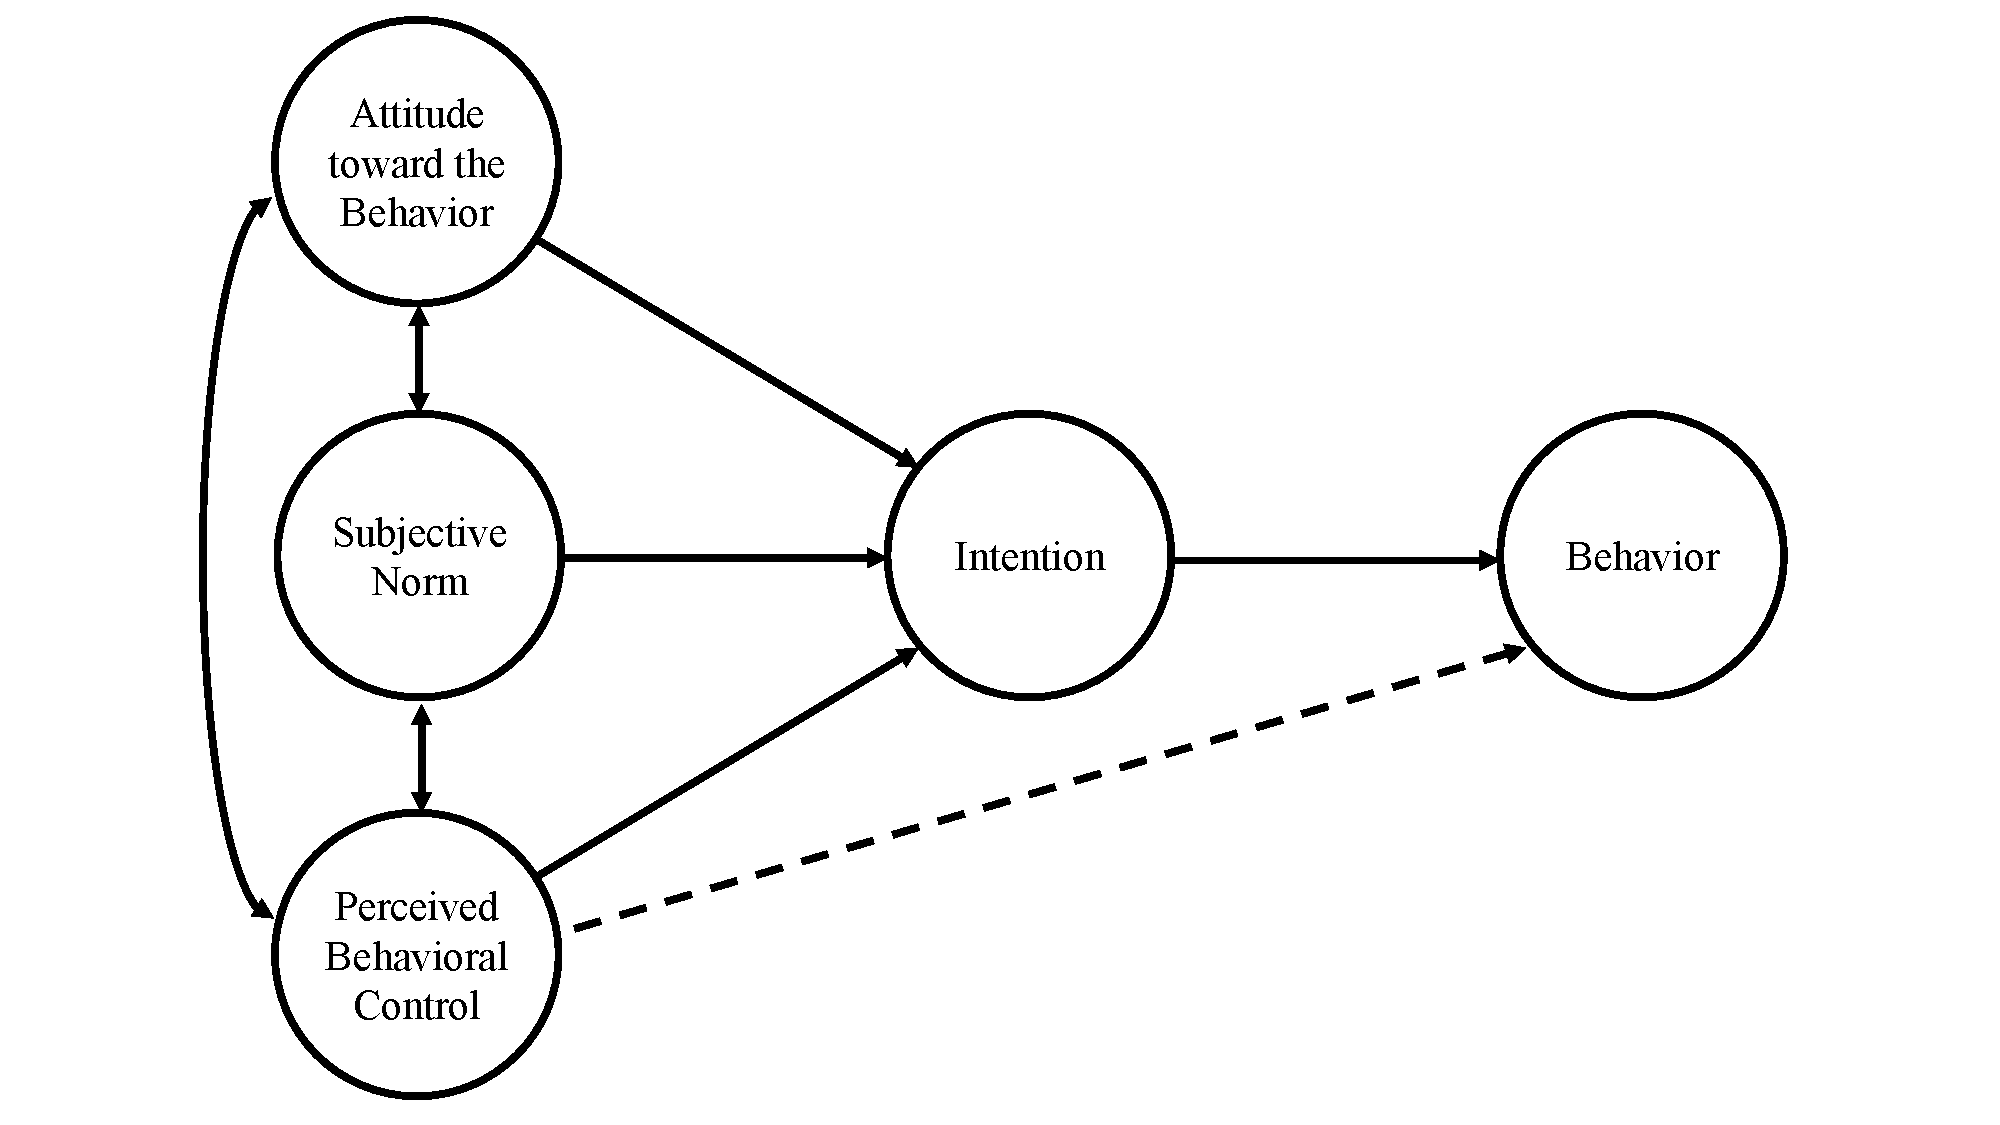
\includegraphics[width=16cm]{images/Ajzen.pdf}
\caption{Theory of Planned Behavior - Source \citep{ajzen1991theory}}
\label{fig:Ajzen}
\end{center}
\end{figure}

Intentions reflect a person's motivation and willingness to engage in efforts to perform the behavior. Thus, the greater the intention, the more likely is the action. From this follows that \acf{ei} is a good predictor of actual behavior. While this relationship is quite natural and obvious, the \ac{tpb} focuses on the question of what influences the intention and how it can be predicted. According to the theory, intentions have three antecedents (see: Figure \ref{fig:Ajzen}): \acf{atb}, \acf{sn} and \acf{pbc}.

\subsection{\acl{atb}}
The \ac{atb} reflects the personal opinion about the behavior and therefore is an internal influence factor \citep{ajzen1985intentions}. When a person is confronted with a new situation that requires action, they can draw from their memories of prior behavior. The former actions and their outcomes are already positively or negatively evaluated and used to build the new attitude.
\citet{ajzen1988attitudes} found a high correlation between \ac{atb} and actual behavior. 
Additionally, he sees high value for predictions in this antecedent, as it can be measured before an action.

\subsection{\acl{sn}}
The \ac{sn} reflects the social pressure imposed on an individual by others, i.e. family, friends or even cultural norms \citep{ajzen1991theory}. Ajzen claims that people assess to what extent their personal influence sphere might approve or disapprove of an action. These are the so called normative beliefs. The \ac{sn} then depends on the normative beliefs and the willingness to adhere to them.
%The \ac{sn} depends on the normative beliefs originating from others and also the willingness to adhere to their opinions.
In contrast to \ac{pbc} and \ac{atb}, \ac{sn} is the only antecedent representing external influences.

\subsection{\acl{pbc}}
The last antecedent is the \ac{pbc}. A person might feel or not feel capable of pursuing an action and therefore is encouraged or discouraged \citep{ajzen1988attitudes}. \ac{pbc} depends on the control beliefs from previous actions and experience from others.
Ajzen prefers the perception over the actual behavioral control. It is understandable that a behavior which is not under one's control due to the lack of resources, personal or other constraints, cannot be pursued. That is why he focused on the perception thereof. In contrast to \ac{sn}, \ac{pbc} is another internal influence factor.
\citet{ajzen1988attitudes} stated that there is a strong correlation between \ac{pbc} and actual behavior. Furthermore, he stressed that the \ac{pbc} is affected by situation and thus differs from the person's general locus of control.

\section{The \acl{tpb} in Entrepreneurship and Hypothesis I}
\label{sec:tpb-literature}
\ac{tpb} was developed for intentions in various settings. Therefore, we put the model in following paragraphs in the context of entrepreneurship in general and \ac{ei} in particular and outline how it is perceived in entrepreneurship literature.
%The \acl{tpb} is considered one of the most famous theories for predicting the entrepreneurial intention. In this section, we outline the perception of the \ac{tpb} in literature as well Shapero's competing model of \acf{see}. Furthermore, a brief comparison of the two models is provided.
%
%\subsection{Competing Model - Shapero's Entrepreneurial Event - delete this?}
%\citet{shapero1982social} introduced the model of \ac{see} for predicting and explaining intentions. Similar to the \ac{tpb}, it also implements three influence factors. "Perceived desirability" describes to what extent an action is considered favorable. "Perceived feasibility" reflects whether a person feels capable of performing the behavior. Finally, the "Propensity to act" is the degree to which a person is inclined to actually engage in the acting.
%
%According to \citet{krueger2000competing}, the two featured models are state of the art in terms of robustness and predictive capability . In their comparison of the two theories, the authors match Ajzen's components \ac{sn} and \ac{atb} to Shapero's "perceived desirability". The authors also state that Shapero's "perceived feasibility" and Ajzen's \ac{pbc} correspond to Bandura's concept of perceived self-efficacy \citep{bandura1986explanatory}. However, Krueger et. al state that people with the possibility to engage in entrepreneurial action might not have the intention to do so. Then on the other side, there are people who want to found a company, but have not launched a business. According to \citet{krueger2000competing}, Shapero's additional antecedent of "propensity to act" accounts for the latter case.

%\subsection{} %is a subsection required here at all?
%In fact, \citet{brannback2006replicate} show that intention is largely dependent on perceived desirability and perceived self-efficacy. According to \citet{fitzsimmons2011interaction} this is the "predominant view". Additionally, \citet{krueger2000competing} see a minor and not significant impact of \ac{sn} on intent. Ajzen himself concluded, that personal characteristics are stronger predictors than the influence of other people \cite{ajzen1991theory}.

\citet{krueger2000competing} mapped the \ac{tpb} components on terms that are more common in the entrepreneurship literature. \ac{pbc} was rephrased as perceived self-efficacy, whereas \ac{atb} and \ac{sn} where together rephrased as perceived desirability. However, they found that \ac{sn} as a factor of perceived desirability has little impact on intent in the entrepreneurial setting. \citet{fitzsimmons2011interaction} even claimed this to be the "predominant view". \citet{ajzen1991theory} himself concluded that depending on the context, personal characteristics might be stronger predictors than the influence of other people.

\citet{fitzsimmons2011interaction} covered the interaction between perceived desirability and perceived self-efficacy in more detail in the entrepreneurial context. According to their paper, either of those influence factors is sufficient to form \acp{ei}. If perceived desirability is high, adding perceived self-efficacy does not significantly add to the score of intention. The same applies to high perceived self-efficacy and low desirability. This is in contrast to the \ac{tpb}. \citet{fitzsimmons2011interaction} referred to this phenomenon in their paper as "natural entrepreneur" (high perceived desirability/high perceived self-efficacy), "accidental entrepreneur" (low/high) and "inevitable entrepreneur" (high/low).

In general, the \acl{tpb} is considered to be state-of-the-art \citep{krueger2000competing}. Even though it was originally not tailored to entrepreneurship, it became one of the most frequently applied theories in the research area of \ac{ei} \citep{fayolle2015impact}. Additionally, the \ac{tpb} is well suited for studies about the influence of \ac{ee} on \acp{ei} \citep{maresch2016impact}.
According to \citet[p. 327]{krueger1993entrepreneurial}, "the theory of planned behaviour demonstrate great utility to social psychologists and thus offer considerable potential for entrepreneurship researchers. For instance, researchers might use this model to analyse how the process of doing a business plan or entrepreneurial training affects intentions."

As a consequence, our hypotheses 1a-1c aim at verifying the \ac{tpb} by providing evidence for the following statements.

\textbf{Hypothesis 1a}: The \acl{atb} positively and significantly effects the person's \acl{ei}.\\
\textbf{Hypothesis 1b}: The \acl{sn} positively and significantly effect the person's \acl{ei}.\\
\textbf{Hypothesis 1c}: The \acl{pbc} positively and significantly effects the person's \acl{ei}.\\
%\subsection{Further general findings about EI based on Ajzen's Model}
%As mentioned in the previous section, \ac{tpb} is popular in science. That is why there are many findings based on this theory. The following paragraph lists some of the most important findings based on \ac{tpb}.
%for example, that social norms have a limited impact
%\begin{itemize}
%\item Bullough, 2014, Importance of Self-efficacy and resiliance for EI
%\item Krueger, Norris F.; Carsrud, Alan L. (1993): Entrepreneurial intentions. Applying the theory of planned behaviour
%\item Linan, Francisco; Chen, Yi-Wen (2009): Development and Cross-Cultural Application of a Specific Instrument to Measure Entrepreneurial Intentions
%\end{itemize}